\section{Random Forest e Dataset KDD'99}

% ------------------------------------------------------------
\subsection{Random Forest: Concetti e Algoritmo}
% ------------------------------------------------------------

Per mitigare i difetti degli alberi decisionali, si
introduce il concetto di \textbf{Random Forest}. I
principali svantaggi dei DT sono l'overfitting e
l'instabilità. Poiché l'accuratezza migliora con ogni
nodo interno, l'addestramento tende a far crescere
l'albero al massimo, modellando il rumore e deteriorando
la capacità di generalizzazione. L'instabilità si
manifesta quando anche piccoli cambiamenti nei dati di
addestramento portano a un albero completamente diverso.

Le Random Forest affrontano entrambi i problemi. L'idea
fondamentale è costruire alberi multipli utilizzando
diversi sottoinsiemi dei dati di addestramento e delle
feature. Per ogni record nella fase di test, le
predizioni vengono aggregate tramite \textbf{voto di
maggioranza} o valore medio. Anche se un albero fa
overfitting sul suo sottoinsieme, gli altri alberi
nella foresta compensano l'errore, poiché sottoinsiemi
diversi producono alberi diversi tra loro.

% ............................................................
\subsubsection{Complessità e Interpretabilità}
% ............................................................

Dal punto di vista della complessità, addestrare una
foresta di $B$ alberi richiede un tempo $B$ volte
superiore rispetto alla costruzione di un singolo albero.
Tuttavia, poiché tutti gli alberi vengono addestrati in
modo indipendente, è possibile costruirli
\textbf{simultaneamente in parallelo}, accelerando
il processo.

Poiché le foreste combinano molti alberi, anche se uno
fa overfitting, è probabile che gli altri non lo facciano.
Ci aspettiamo che un ensemble sia più accurato e più
propenso a fornire la classificazione corretta. Tuttavia,
le foreste \textbf{perdono l'interpretabilità} tipica
di un singolo albero.

% ............................................................
\subsubsection{Bagging e Randomizzazione delle Feature}
% ............................................................

L'algoritmo Random Forest combina due metodi principali per 
risolvere overfitting e instabiilità:

\begin{itemize}
    \item \textbf{Bagging (Bootstrap Aggregation)}:
        campionamento dei dati \textit{con sostituzione}.
        Riduce la varianza dei campioni, pur introducendo
        discenti deboli (\textit{weak learners}); il bias
        introdotto viene poi ridotto tramite l'ensembling.
        La probabilità che un campione sia in ds originale e
        non nel bootstrappato è
        $\approx 1/e \approx 0.37$ (37\%).
    \item \textbf{Selezione casuale delle feature}:
        rimuove la correlazione tra gli alberi. Ad ogni
        punto di divisione si considera un sottoinsieme
        casuale di $M$ attributi invece dell'intero set
        di $P$ attributi, permettendo di selezionare
        anche attributi non dominanti.
\end{itemize}

\begin{figure}[H]
    \centering
    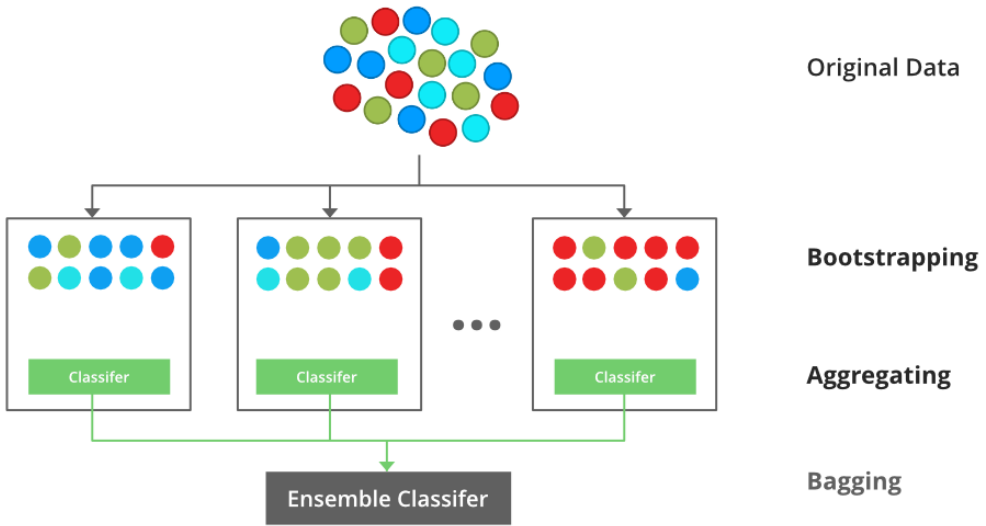
\includegraphics[width=0.7\textwidth]{img/randomForest.png}
\end{figure}

Dai dati originali si creano diversi campioni tramite Bootstrapping
(Campionamento con Rimpiazzo). Ogni capione addestra un 
Classificatore separato. Infine i risultati vengono aggregati per 
formare il \textbf{Classificatore Ensenble}

La motivazione matematica della feature randomization
si basa sulla varianza di una combinazione di alberi.
Dati $B$ alberi con varianza $\sigma^2$ e correlazione
a coppie $\rho$, la varianza dell'ensemble è:

\begin{equation}
    Var(f) = \rho\,\sigma^2
    + \frac{1-\rho}{B}\,\sigma^2
\end{equation}

Quando $B \to \infty$, si ottiene $Var(f) = \rho\,\sigma^2$.
Riducendo la correlazione $\rho \to 0$ tramite la
randomizzazione delle feature, si ottiene
$Var(f) \to 0$, ovvero la varianza dell'ensemble
tende a zero.

Se le caratteristiche disponibili al punto di divisione sono p=4, l'
algoritmo selezona casualmente m = $\sqrt{P} = 2$ candidati per la divisione.
Questo assicura che ogni albero si concentri su aspetti diversi dei dati, 
evitando di usare sempre le stesse caratteristiche dominnanti e decorrelando
così gli alberi.

Selezionando la carateristica per la divisione tra quelle randomizzate,
si riduce l'influenza delle caretteristiche dominanti.


% ------------------------------------------------------------
\subsection{Il Dataset KDD'99: Struttura e
Pre-Processamento}
% ------------------------------------------------------------

Per l'applicazione pratica delle tecniche descritte, si
utilizza il \textbf{dataset KDD'99}. Esso contiene molti
attacchi raggruppati in 5 classi di traffico:

\begin{itemize}
    \item \textbf{Benign Traffic}: traffico normale.
    \item \textbf{Denial-of-Service (DoS)}: attacchi che
        saturano le risorse del sistema.
    \item \textbf{Network Probe (Probe)}: scansioni
        della rete per individuare vulnerabilità.
    \item \textbf{Remote-to-Local (R2L)}: tentativi di
        accesso remoto non autorizzato.
    \item \textbf{User-to-Root (U2R)}: escalation di
        privilegi locali.
\end{itemize}

Esiste un pattern noto di escalation: un attacco spesso
evolve da Probe a R2L fino a U2R.

Il dataset presenta feature suddivise in due categorie.
Le \textbf{feature note} includono: durata della sessione,
tipo di protocollo, servizio, flag, byte sorgente/dest.,
frammenti errati e pacchetti urgenti. Le
\textbf{feature aggiuntive} legate al servizio includono
i tassi di errore (REJ o SYN/S0) e le percentuali di
connessioni agli stessi o diversi servizi.

% ............................................................
\subsubsection{Esperienza Operativa e Riduzione Feature}
% ............................................................

L'esperienza empirica con il dataset KDD'99 ha evidenziato
diverse criticità. Una classificazione diretta delle
singole classi può fornire risultati scadenti, con
una problematica comune nell'errata classificazione
degli errori. Si rende quindi necessaria una
\textbf{riduzione delle feature} per rimuovere la
ridondanza, idealmente con perdita di prestazioni
nulla o minima.

Per il pre-processamento dei dati, le tecniche valutate
producono risultati differenti:

\begin{itemize}
    \item \textbf{StandardScaler}
        ($Y = \frac{X - \mu}{\sigma}$): non fornisce
        benefici tangibili.
    \item \textbf{MinMaxScaler}
        ($y = \frac{X - X_{min}}{X_{max} - X_{min}}$):
        non apporta vantaggi significativi.
    \item \textbf{RobustScaler} (raccomandato): sfrutta
        l'intervallo interquartile (IQR 75-25):
\end{itemize}

\begin{equation}
    y = \frac{X - \text{median}(X)}{IQR}
\end{equation}

Il RobustScaler è preferibile in quanto la mediana è
statisticamente meno suscettibile agli outlier rispetto
alla media. La matrice di correlazione (heatmap) mostra
che pochissime feature sono fortemente correlate tra
loro, portando a una riduzione trascurabile della
dimensionalità.

% ------------------------------------------------------------
\subsection{Approcci Sperimentali e Classificazione
Gerarchica}
% ------------------------------------------------------------

Nel corso delle sperimentazioni sono stati testati
diversi approcci di Machine Learning sul dataset KDD'99:
Decision Tree, k-NN, SVM (kernel lineare e RBF),
Random Forest e reti neurali. Le prestazioni variano
significativamente tra i metodi.

Focalizzandosi sul \textbf{k-NN} con $K=5$ e
pre-processamento tramite Robust Scaling, si ottengono
le migliori prestazioni in termini di accuratezza.
Tuttavia, molti attacchi DoS vengono erroneamente
classificati come Probe, e le prestazioni per R2L e U2R
sono molto scarse. Il problema principale è il
\textbf{tempo di test}: circa 40 minuti per processare
il dataset di test (25.000 righe), corrispondenti a
$\approx 10$ ms per singola istanza — una latenza
eccessiva per applicazioni real-time.

Esaminando le \textbf{SVM}, si nota che convergono
solo applicando la normalizzazione. I tempi variano
drasticamente in base al kernel:

\begin{table}[h!]
\centering
\begin{tabular}{lll}
\toprule
\textbf{Kernel} &
\textbf{Training} &
\textbf{Test (per istanza)} \\
\midrule
LinearSVC &
30 sec &
$4.5\,\mu$s \\
RBF &
11 min &
$6.0$ ms \\
\bottomrule
\end{tabular}
\caption{Confronto tempi SVM per kernel}
\end{table}

% ............................................................
\subsubsection{Alternativa: Classificazione a Due Stadi (Gerarchica)}
% ............................................................

Considerando le limitazioni degli approcci a singolo
stadio, è stata proposta una
\textbf{classificazione gerarchica a due stadi}:

\begin{enumerate}
    \item \textbf{Primo stadio}: distingue tra attacco
        e non-attacco, basandosi su principi di
        \textit{anomaly detection}. Implementato con
        DT o RF abbinati al Robust Scaling, garantisce
        accuratezza molto alta e falsi positivi/negativi
        molto bassi (solo 36 falsi negativi e 183 falsi
        positivi su grandi volumi).
    \item \textbf{Secondo stadio}: discrimina le
        tipologie specifiche di attacco non risolte
        dal primo stadio (\textit{misuse detection}).
        Rimane un problema aperto.
\end{enumerate}

La ripartizione del dataset per il sistema gerarchico
è la seguente:

\begin{table}[h!]
\centering
\begin{tabular}{lll}
\toprule
\textbf{Stadio} &
\textbf{Training} &
\textbf{Testing} \\
\midrule
Singolo stadio &
253.333 &
214.333 \\
Livello 1 (gerarchico) &
253.333 &
214.333 \\
Livello 2 (solo attacchi) &
176.911 &
85.997 \\
\bottomrule
\end{tabular}
\caption{Distribuzione del dataset KDD'99}
\end{table}

Il secondo livello riceve in input solo le istanze
classificate come attacco dal primo stadio, riducendo
il volume dei dati a circa un terzo rispetto al
singolo stadio.

% ............................................................
\subsubsection{Confronto Algoritmi al Secondo Livello}
% ............................................................

Analizzando le prestazioni al secondo livello della
classificazione gerarchica, emergono differenze tra
gli algoritmi:

\begin{itemize}
    \item \textbf{Random Forest (RF)}: buona
        concentrazione sulla diagonale per DoS e Probe,
        ma difficoltà sulle classi minoritarie.
    \item \textbf{Linear SVM}: comportamento simile
        a RF, con distribuzione degli errori leggermente
        diversa sulla classe DoS.
    \item \textbf{RBF SVM}: buona capacità sulle classi
        maggioritarie, ma con le criticità temporali
        già discusse.
    \item \textbf{k-NN ($K=5$)}: efficace per accuratezza
        (DoS: 81.346 corretti, Probe: 1.268 corretti),
        ma tempo di testing di 630 secondi
        ($\approx 7.4$ ms per istanza), ancora troppo
        lento per uso real-time.
\end{itemize}

In conclusione, nessun singolo algoritmo risolve
perfettamente tutte le classi. L'approccio gerarchico
con RF al primo livello e un algoritmo dedicato al
secondo rappresenta la soluzione con il miglior
compromesso tra accuratezza e prestazioni temporali.
